\documentclass{article}
\usepackage{amsmath}
\usepackage{graphicx}
\usepackage[utf8]{inputenc}
\usepackage[bahasai]{babel}
\usepackage{array}
\usepackage{float}

% title
\title{Matematika 1}
\author{Y. Susatio \& B.T. Atmaja\\
\emph{Department of Engineering Physics}\\
Institut Teknologi Sepuluh Nopember}
\date{\today}

\numberwithin{equation}{section}
\begin{document}
\maketitle

\section{Persamaan Garis}
\subsection{Bentuk Umum Persamaan Garis}
Bentuk umum persamaan garis lurus adalah sebagai berikut,
\begin{equation}
    ax+by+c = 0
\end{equation}

dimana a, b, c adalah bilangan real.\\
Ubah persamaan diatas menjadi:
$$ by = -ax -c$$ 
Jika kesemua sukunya dibagi dengan $b$ maka,
$$ y = -\frac{a}{b}x - \frac{c}{b}$$
dimana $\cfrac{a}{b}$ merupakan gradien garis = $\tan \theta=m$\\
$\theta$ = sudut positif antara garis dan sumbu x.\\
\vskip10pt
\begin{tabular}{ l c r }
\raisebox{-.5\height}{\includegraphics[width=2in]{pict/m1}} & & $m = \dfrac{y_B-y_A}{x_B-x_A}=\dfrac{y_A-y_B}{x_A-x_B}$
\end{tabular}

\subsection{Persamaan Garis Lewat ($x_0, y_0$) dengan gradien $m$}
\begin{equation}
    y-y_0=m(x-x_0) \label{pers1_2}
\end{equation}

\subsection{Persamaan garis lewat dua titik($x_a, y_a$), ($x_b, y_b$)}
Gunakan persamaan \ref{pers1_2} untuk memperoleh persamaan garis lewat dua titik sebagai berikut dengan mensubtitusi nilai m menjadi sebagai berikut,
$$y - y_A = \dfrac{y_B - y_A}{x_B - x_A} (x - x_A)$$
\begin{equation}
\dfrac{y-y_B}{y_B - y_A} = \dfrac{x - x_A}{x_B - x_A}
\end{equation}

\subsection{Sudut antara dua garis}
Jika diketahui dua garis, $g$ dan $l$, dimana persamaan keduanya adalah sebagai berikut, \\
$g: \hskip10pt ax + by + c = 0 \rightarrow m_1= - \dfrac{a}{b} $ \\ \\
$l: \hskip10pt px + qy + r = 0 \rightarrow m_2= - \dfrac{p}{q} $ \\ \\
maka sudut antar dua garis tersebut dapat dicari dengan persamaan berikut:\\
$$ \tan \theta = \dfrac{m_2 - m_1}{1+m_1m_2} ~~\Longrightarrow~~Buktikan!!$$

\subsection{Jarak titik($x_0, y_0$) ke garis $ax+by+c=0$} 
Jika $d$ adalah jarak dari titik ($x_0, y_0$) ke garis  $ax+by+c=0$, maka $d$ dirumuskan, \\
\begin{equation}
    d = \Biggl|\dfrac{a.x_0+b+y_0+c}{\sqrt{a^2+b^2}} \Biggr|
\end{equation}

\subsection{Persamaan garis bagi sudut}
Jika diketahui dua gari, $g$ dan $l$, seperti sebelumnya,\\
$g: \hskip10pt ax + by + c = 0 $ \\ 
$l: \hskip10pt px + qy + r = 0 $\\ \\
maka persamaan garis bagi sudut dinyatakan dengan \\
\begin{equation}
    \dfrac{ax+by+c}{\sqrt{a^2+b^2}} = \dfrac{px+qy+r}{\sqrt{p^2+q^2}}
\end{equation}

\subsection{Persamaan berkas garis}
Kembali kita menggunakan dua persamaan gari sebagai berikut, \\
$g: \hskip10pt ax + by + c = 0 $ \\ 
$l: \hskip10pt px + qy + r = 0 $\\ 
Setiap garis yang melewati titik potong kedua garis tersebut, disebut sebagai persamaan berkas garis,
\begin{equation}
    \fbox{$g+\lambda{l} = 0$}
\end{equation}
dimana $\lambda$ = konstanta yang ditentukan dari syarat sebelumnya.

\subsection{Pergeseran grafik}
\underline{Pergeseran ke kanan - kiri} \\
Perhatikan persamaan garis lurus di bawah ini,\\
\begin{figure}[!h]
\begin{center}
    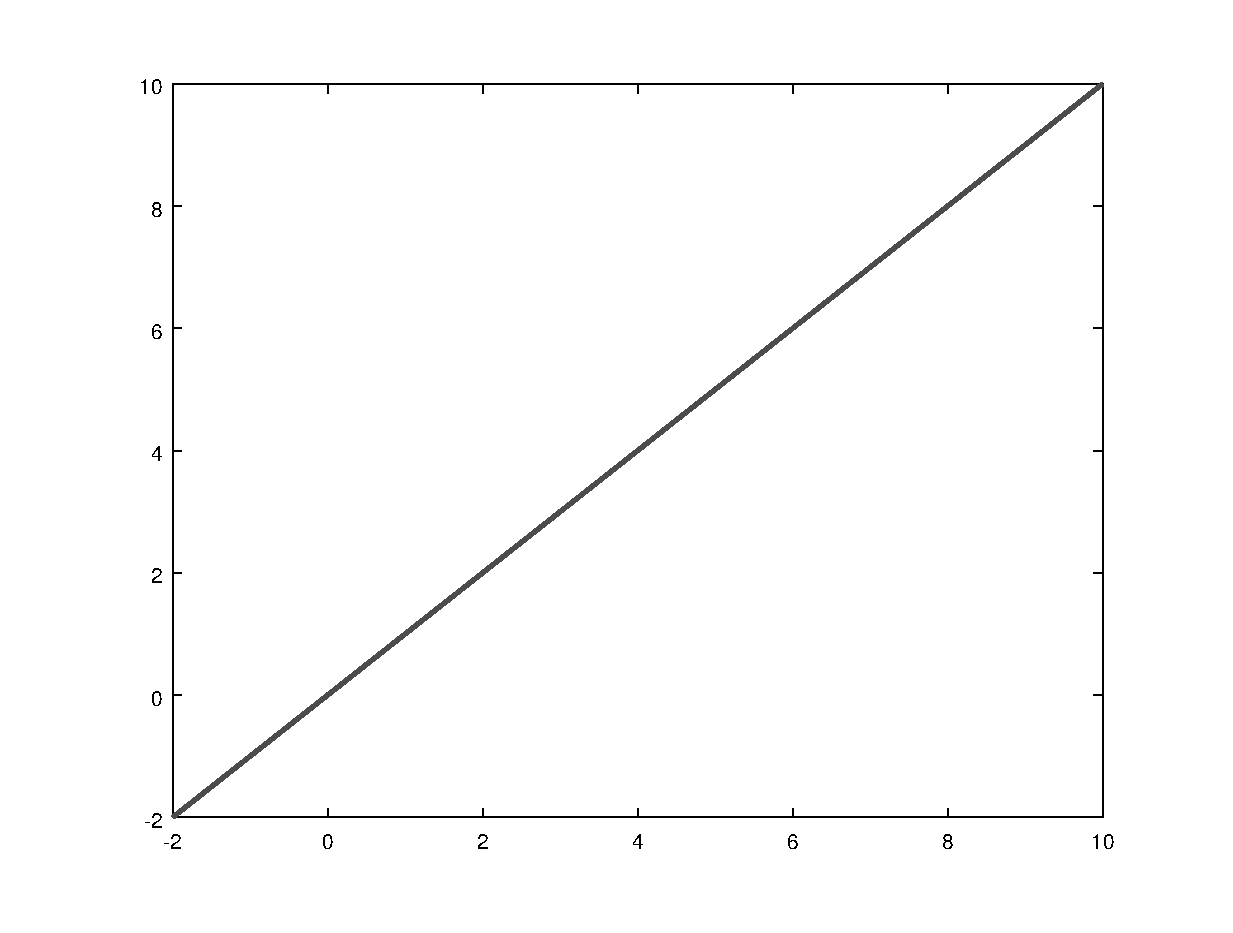
\includegraphics[width=3in]{pict/grafik1}
    \caption{Grafik persamaan garis $y=x$} \label{grafik1}
\end{center}
\end{figure}
Jika setiap titik pada garis tersebut digeser $//$ sumbu x kekanan sejauh 2, maka akan didapatkan pergeseran grafik seperti pada gambar \ref{grafik1-2}\\
\begin{figure}
\begin{center}
    \includegraphics[width=3in]{pict/grafik1-2}
    \caption{Grafik persamaan garis $y=x-2$} \label{grafik1-2}
\end{center}
\end{figure}
 \\
asal: $y = x$ \\
Hasil geser:    $y= x-2 $\\
$x \rightarrow (x-2)$\\
$y - 0 = 1(x -2)$\\
$y = x - 2$\\

Jadi pergeseran kekanan sejauh 2, terjadi jika
\begin{center}
    $x \rightarrow (x-2)$
\end{center}


\underline{Soal:}

Garis $y=x+5$ terbentuk jika $y=x$ digeser ke .... sejauh .....\\
 \\
\underline{Pergeseran ke atas - bawah}\\
$y=x$ digeser menjadi $y=x-2$ atau $y+2=x$\\
yang berubah $y \rightarrow (y+2) \Longrightarrow$ digeser ke bawah sejauh 2\\

\begin{figure}[!h]
\begin{center}
    \includegraphics[width=3in]{pict/grafik1-3}
    \caption{Grafik persamaan garis $y+2=x$} \label{grafik1-3}
\end{center}
\end{figure}

Pergeseran tersebut berlaku untuk fungsi-fungsi lain $y=f(x)$.

\underline{Soal}
\begin{enumerate}
    \item Gambarlah: \\
        a. $y = x^2$ \\
        b. $y = (x-1)^2$ \\
        c. $y = (x-1)^2 - 4$
    \item $y = 2 \cos(3x+\dfrac{\pi}{2})$ diperoleh dengan menggeser grafik $y = 2 \cos (3x)$ ke ... sejauh ...
    \item Dapatkan persamaan kurva berikut:
\begin{center}
    \includegraphics[width=4in]{pict/triangle.png}
\end{center}
\end{enumerate}

\section{Grafik Parabola}
\subsection{Parabola dengan sumbu simetri sejajar sumbu $x$}
\underline{Definisi:} Parabola adalah tempat kedudukan titik-titik yang berjarak sama terhadap satu titik dan satu garis.\\
Titik tersebut adalah fokus.\\
Garis tersebut adalah direktrik. \\ \\

\begin{center}
\includegraphics[width=3in]{pict/parabola3}
\end{center}

Agar $A(x,y)$ berada pada parabola (sesuai definisi) maka $d_1=d_2$, \\ \\
$d_1 = \sqrt{(x-P)^2 + (y - 0)^2}$ \\
$d_2 = (x+p)$ \\
$(x+p) =  \sqrt{(x-P)^2 + y ^2}$ \\
$(x+p)^2 = (x-p)^2 + y^2$ \\
$ x^2 + 2xp + p^2 = x^2 - 2xp + p^2 + y^2$ 
\begin{equation}
 y^2 = 4px 
\end{equation}
$\Longrightarrow$  Persamaan parabola dengan puncak (0,0) \\
\hspace*{16px} Fokus (P,0) direktrik, $x=-p$. \\
\\
Ubah cara menyatakan parabola tersebut menjadi, \\
$(y-0)^2 = 4p(x-0) \Rightarrow puncak(0,0)$ \\
Jika grafik tersebut punyaknya digeser ke (a,b) maka persamaannya menjadi, 
\begin{equation}
    (y-b)^2 = 4p(x-a)
\end{equation}
$F(P+a, b)$ \\
Direktrik $x=-p + a$, sumbu simetri $y=b$. \\ \\
\underline{Soal:} \\
Dapatkan puncak, fokus dan persamaan direktrik dari $y^2 - 4y - 8x -4 =0$ \\
Catatan: Jika $p > 0$ maka grafik terbuka ke kanan, \\
\hspace*{39px} Jika $p<0$ maka grafik terbuka ke kiri.

\subsection{Parabola dengan sumbu simetri sejajar sumbu $y$}
\begin{center}
\includegraphics[width=3in]{pict/parabola4}
\end{center}
Agar $A(x,y)$ berada pada parabola (sesuai definisi) maka $d_1=d_2$, \\ \\
$d_1 = \sqrt{(x-0)^2 + (y - P)^2}$ \\
$d_2 = (y+p)$ \\
$\sqrt{x^2 + (y-P) ^2} =(y+p) $ \\
${x^2 + (y-P) ^2} =(y+p)^2$ \\
$ x^2 + y^2 -2yp + p^2 = y^2 + 2yp + p^2 $ \\ \\
\begin{equation}
4py = x^2 \longrightarrow \fbox{$y=\dfrac{1}{4P}x^2$}
\end{equation}
$\Longrightarrow$ Persamaan parabola dengan sumbu simetris $//$ sumbu y. \\
 \hspace*{16px}  Fokus (0,P) direktrik, $y=-p$. \\
\vspace*{10pt}
$$(y-0) = \dfrac{1}{4P} (x-0)^2 \Longrightarrow ~~Puncaknya~~(0,0)$$ \\
Jika puncaknya (a,b) maka persamaannya, \\
\begin{equation}
(y-b) = \dfrac{1}{4P} (x-a)^2 \\
\end{equation}
Fokus: $F(a,b+p)$ \\
Direktrik: $y=-p+b$  \\
Sumbu simetris $x=a$.
\vskip20pt
\underline{Soal:}
\begin{enumerate}
\item Dapatkan F, direktrik dan sumbu simetris dari:
    \begin{enumerate}
    \item $y=x^2 - 6x+ 14$
    \item $y=4x^2 - 4x -3$
    \end{enumerate}
\item Buatlah sketsa dari grafik:
    \begin{enumerate}
    \item $y=x^2 - x - 6$
    \item $y=12 - x - x^2$
    \item $y=x^2 + x + 5$
    \item $y=-x^2 +x-9$
    \end{enumerate}
\end{enumerate}

\subsection{Bentuk lain persamaan parabola}
$$ y = ax^2+bx+c ~~~\Longrightarrow~~~a,b,c = real, a\neq 0$$
\begin{equation}\label{parabolaLain}
\begin{split}
y &= a\bigl[x^2+\dfrac{b}{a}x+\dfrac{c}{a}\bigr] \\
  &= a\Bigl[x^2+2x \Bigl\{\dfrac{b}{2a}\Bigr\}+\Bigl\{\dfrac{b}{2a}\Bigr\}^2-\Bigl\{\dfrac{b}{2a}\Bigr\}^2+\dfrac{c}{a}\Bigr] \\
  &= a\Bigl[\Bigl(x+\dfrac{b}{2a}\Bigr)^2-\Bigl(\dfrac{b^2-4ac}{4ac^2}\Bigr)\Bigr]\\
y &= a\Bigl(x+\dfrac{b}{2a}\Bigr)^2-\dfrac{D}{4a}
\end{split}
\end{equation}

Koordinat puncak $\Bigl(-\dfrac{b}{2a}, -\dfrac{D}{4a}\Bigr)$\\

\underline{Soal:}
\begin{enumerate}
\item Dapatkan persamaannya!
\begin{figure}[H]
\includegraphics[width=2.7in]{pict/parabolaSoal1}
\end{figure}
\item Dapatkan persamaannya!
\begin{figure}[H]
\includegraphics[width=3in]{pict/parabolaSoal2}
\end{figure}
\item A(2,1); B(10,6); C(4,12). Dapatkan luas segitiga ABC.
\end{enumerate}

\end{document}
